% This file is isea.tex. It contains the formatting instructions for and acts as a template for submissions to ISEA 2025. It is based on the ICCC formats and instructions. It uses the files isea.sty, isea.bst and isea.bib, the first two of which also borrow from AAAI IJCAI formats and instructions.
% Modified from ICCC.tex by B. Bogart

\documentclass[letterpaper]{article}
\usepackage{isea}
\usepackage[pdftex]{graphicx}
\usepackage{times}
\usepackage{helvet}
\usepackage{courier}
\usepackage[numbers]{natbib}
\pdfinfo{
/Title (Towards an Effective Theory of Art)
/Author (Kynan Stewart Hughes)}
% The file isea.sty is the style file for ISEA 2025 proceedings.
%
\title{Towards an Effective Theory of Art}
\author{Kynan Stewart Hughes\\
Creativity and Cognition Studios\\
University of Technology Sydney\\
Sydney, Australia\\
kynan.s.hughes@student.uts.edu.au\\
\newline
\newline
}
\setcounter{secnumdepth}{0}

\begin{document} 
% Setting the default tolerance level
% \tolerance=200
% Setting a high tolerance level
% \tolerance=10000
% Some more drastic measures for hbox issues
% \emergencystretch=4em
% \raggedright
\maketitle
\begin{abstract}
The Proceedings of the International Symposium on Electronic
Art will be compiled from electronic manuscripts submitted by
the authors. This paper provides brief style instructions that will
facilitate high-quality, consistent, proceedings. The title
``Abstract'' should be 10 point, bold type, centred at the
beginning of the left column. The body of the abstract
summarizing the thesis and conclusion of the paper in no more
than 200 words should be 9 point, justified, regular type.
\end{abstract}

\keywords{Keywords}

Art, technology, complexity.

\section{Introduction}

    The term \emph{complexity thinking} expresses a sense of complexity as an intrinsic quality shared by diverse phenomena, and a sense of things being connected in unpredictable ways. The term acknowledges, according to Paul Cilliers and Kurt Richardson, the “...epistemological consequences of assuming the ubiquity of complexity” \citep{CilliersRichardsonCmplxtyScnc2001}. Complexity thinking describes an awareness that we can never fully know the dynamic interconnected processes at play within and between all phenomena. While it limits what we can reasonably claim to know, it also changes how we think about the world in ways that create new possibilities for knowing. 

    Complexity thinking connects diverse modes of developing theory and practice. Gradually over the last 80 years, and more quickly since the late 1970s, the idea of complexity has shifted scientific thinking away from a deterministic, mechanical model of reality and towards a view in which the world consists of interconnected, non-deterministic systems operating at every scale. In the humanities, the tradition of process philosophy was given new energy by Deleuze and Guattari, and has morphed into New Materialism, Speculative Realism and Post-humanism. DeLanda's Assemblage Theory functions as a streamlined, operationalisable synthesis of Deleuze and Guattari. Brian Massumi's idea of \emph{affect} supersedes cause and effect, and grounds science and art in the same processes of complex mutual interaction. Jason Hoelscher's Complex Adaptive Systems aesthetics synthesises scientific theories of complex systems with the process philosophy of Gilbert Simondon, to produce a coherent and materialist theory of art.

    An effective theory is one that is “...able to organize phenomena under an efficient set of principles...” and is also “...not impossibly complex...” \citep[p.1]{WellsEffctvThrs2012}. A good effective theory functions as a heuristic — a rule of thumb that can serve as a guide for action. An effective theory need not be true — the critical requirement is \emph{observational consistency} \citep[p.71]{WellsEffctvThrs2012}.

    This paper proposes an effective theory for art — namely that art is a technology, or at least may be usefully treated as one. This conclusion is derived from a comparison of Brian Arthur's theory of technology which is based largely on Complex Adaptive Systems Theory, and Jason Hoelscher's theory of art objects as complex adaptive systems, which draws from Process Philosophy — especially Gilbert Simondon's work on the technology.

    % Generally speaking, it is more important for an effective theory to be fit for purpose than that it be, for example, falsifiable, simple or analogous with other theories \citep[pp.61–68]{WellsEffctvThrs2012}, although it may have those qualities.

    % In \emph{Inventing Temperature}, Hassock Chan called William Thompson's reliance on an unproven theory \emph{heuristic}: “Thomson [...] had serious doubts about [the theory's] rigorous truth. In fact, [...] he considered [it] an as-yet unverified hypothesis. However, he thought [it] was probably approximately true, and therefore capable of serving as a point of departure [...] . Thus, Thomson used [it] as a heuristic device” [...] \citep[p.185]{ChangInvntngTmprtr2004}

\section{Technology}

    According to Brian Arthur, the economist and complexity theorist, a technological object is always “...a means to fulfil a human purpose...” \citep[p.28]{theNatureOfTechnology2009}. A specific technology in this sense is always “...a phenomenon captured and put to use.”\footnote{
        He also expressed it as “...a programming of phenomena for a purpose.” \citep[p.53]{theNatureOfTechnology2009}
    } \citep[p.53]{theNatureOfTechnology2009}. This is a powerful distillation that holds for the full range of diverse technologies, contemporary and historical.

    \begin{quote}
        [...] a technology may be a method or process or device: a particular speech recognition algorithm, or a filtration process in chemical engineering, or a diesel engine. It may be simple: a roller bearing. Or it may be complicated: a wavelength division multiplexer. It may be material: an electrical generator. Or it may be nonmaterial: a digital compression algorithm. Whichever it is, it is always a means to carry out a human purpose\footnote{
            Arthur seems to have been assuming that only humans have technologies. Tool use in animals is very well documented \citep{BeckAnmlTlUs2011} and would certainly qualify as technology according to this definition. \citep[p.28]{theNatureOfTechnology2009} but we will focus on human technologies here.
        }.
    \end{quote}

    Phenomena don't have to be physical phenomena like fire or electricity. They may be “...behavioural or organisational ‘effects’...” \citep[p.55]{theNatureOfTechnology2009} or “...truism[s] of nature...” \citep[p.45]{theNatureOfTechnology2009} (any \emph{regularity}, as Flack would say). 

    [A bit about Jessica Flack's work on coarse graining and emergence]

    A monetary system, for example, is a technology.

    \begin{quote}
        Money is a means to the purpose of exchange, and therefore qualifies as a technology. [...] Its principle is that any category of scarce objects can serve as a medium for exchange: gold, government-issued paper, or when these fail, cigarettes and nylons. The monetary system makes use of the “phenomenon” that we trust a medium has value as long as we believe that others trust it has value and we believe this trust will continue in the future. \citep[p.55]{theNatureOfTechnology2009}
    \end{quote}

\section{The Aesthetic Regime of Art}

    It is necessary to clarify what is meant by ‘art’, because the term is regularly used in a few different ways. I do not mean ‘art’ in the broadest, most general sense, as in ‘the art of war’ or as if I were to say that my car mechanic is a real artist because of her skill and the care she shows in her work. Nor do I mean ‘art’ in the sense of ‘the arts’, as in ‘the arts and sciences’. I mean ‘art’ in the sense of ‘artworks’ as the things that artists make and of which we might say, ‘I don't know much about art, but I know what I like’ - or even (and especially), ‘that thing you just made me look at is NOT art’. I mean the objects that are displayed in art galleries, bought and sold as artworks, written about in art magazines and art history books, and taught about in art schools. I also mean the practices, discourses, institutions, markets and other cultural aspects that constitute the ‘art world’.

    The other senses of ‘art’ — art in the general sense as in “the art of war”, and in the sense of ”the arts”, are not irrelevant because, taken together, all the senses of ‘art’ operate as a set of coexisting, nested meanings and are interconnected aspects of the contemporary global, Westernising culture most of us share to some extent — and let's call that “Modernity” for convenience. I am a practitioner of a kind of Contemporary Art that involves the use of emerging technologies, but I am also practising in the context of academic research that crosses certain boundaries between the arts and the sciences, so I am aware of those boundaries, and I might occasionally congratulate myself for being a real artist in the sense that I am skilled and careful in my work.

    The idea of there being a qualitative difference between the practice we now call ‘the arts‘ and other kinds of crafting began taking shape during the Renaissance\footnote{Reference needed, e.g. Tatarkiewicz, 1971} and by the late 17th century the classification of various practices within the category of ‘the arts’ had become a hot topic in European intellectual circles. This was the Enlightenment, and the craze for categorisation was in full swing. There were many proposals put forward. Batteux’s treatise for example, separated what he called the ‘fine arts’ — music, poetry, painting, sculpture, and dance — from the ‘mechanical arts’. He believed that the fine arts sought to imitate nature (but only its beautiful aspects), and that the fine arts’ sole purpose was to give pleasure. Eloquence and architecture combined pleasure and usefulness, so they were placed in a separate group\footnote{Reference needed, e.g. Kristeller, 1952} \citep[p.632]{NadalSkovAFrwllTArt2020}.

    According to Rancière, the plane on which this qualitative difference emerged, the principle that came to organise these ‘...ways of doing, making, seeing, and judging...’, this ‘...fold in the distribution of ways of doing and making...’, was the ‘...notion of representation or \emph{mimesis}...’. He called this partitioning of the sensible the \emph{regime of representation}\citep[p.22]{RancierPltcsOfThAsthtcs2004}. It is not, in itself, an artistic process, but ‘...a fold that renders the arts visible.‘ It is  ‘...a regime of visibility regarding the arts.’ We still observe this fold of difference. For example, we organise our institutions of learning — our university faculties and school curriculums — along it: science, technology, engineering and maths on one side, the arts and humanities on the other. We wonder how to get more girls to choose STEM subjects in school.

    At the same time the fine arts become recognisable as such, they became bound to ‘...a general order of occupations and ways of doing and making.’ At this time in history, Rancière thought, ‘...the logic of representation, [...] enters into a relationship of global analogy with an overall hierarchy of political and social occupations‘. The various \emph{arts} existed — understood as forms of knowledge and their applications — but they were not recognised as part of a singular, overarching category of human experience. The arts — music, literature, sculpture, painting, et cetera — were disparate practices serving different social functions, and were situated within a stratified system that categorised both activities and the individuals engaged in producing them. The concept of art as a unified field was absent.
    
    \begin{quote}
        Art as we name and understand it in our societies — Art in the singular, with a capital A — was unknown to those who enjoyed themselves at the theatre, commissioned works from painters and sculptors, listened to religious concerts, or hired musicians for their feasts or ceremonies. This is not a merely lexical issue. Art did not exist as a common sphere of experience, not only because the practice of the arts was intended for different social purposes, but, above all, because these purposes were themselves part of a hierarchical division of human activities and of the human beings who engaged in them. \citep[p.25]{RanciereMdrnTms2022}
    \end{quote}

    The regime of representation is epitomised for Rancière by classical theatre, in which the two meanings of the word sense — sensing as in experiencing, and making sense as in to understand conceptually — are tightly coupled.

    \begin{quote}
        The stage was thought of as a magnifying mirror where spectators could see the virtues and vices of their fellow human beings in fictional form. And that vision in turn was supposed to prompt specific changes in their minds: Molière’s Tartuffe supposedly taught spectators to recognize hypocrites; Voltaire’s Mahomet to fight for tolerance against fanaticism, and so on. Now, that ability to produce the dual effect of intellectual recognition and appropriate emotion was itself predicated on a regime of concordance inherent in representation.
    \end{quote}

    Rancière calls the current regime of art, art as we know it, the \emph{aesthetic regime}. The aesthetic regime is superimposed upon, without replacing, the regime of representation and the ethical regime of images \citep[p.50]{RancierPltcsOfThAsthtcs2004}. It is not a single coherent paradigm, but a “plurality” of “...frequently different, and sometimes contradictory, ways of thinking...” \citep[p.8]{RanciereMdrnTms2022} organised around the idea of aesthetic experience. This is a radical repositioning of Aesthetics as art itself, rather than as a theory about art.
    
    The aesthetic regime emerged at the end of the eighteenth century with Emanuel Kant's \emph{Critique of Judgement}. Kant's radical break was to propose that the essence of an art object lies in its capacity to be experienced without concept. With the clarity of hindsight, we can see as Rancière did, that it is the separation of sense-as-in-sensation and sense-as-in-making-sense which created our current situation in which the effectiveness of an artwork, the very thing that makes it art, is (as Rancière put it) “... a paradoxical kind of efficacy that is produced by the very rupturing of any determinate link between cause and effect.” \citep[p.51]{RancierThEmncptdSpcttr2009} ”It is precisely this indeterminacy”, he said, “that Kant conceptualized when he defined the beautiful as ‘what is represented as an object of universal delight apart from any concept’. \citep[p.52]{RancierThEmncptdSpcttr2009}

    The purpose of an artwork must always now be organised around aesthetic experience. This constraint is the origin of art's autonomy within Modernity and the source of all possibility with respect to how art can interact with other aspects of Modernity, including all potential for generating meaning or taking political action, for example. All distinctions and differences within the idea of art operate within the aesthetic regime. Ideas about Modern and Post-Modern art, for example, are simply different, perhaps contradictory strategies for trying to do something worth doing within the aesthetic regime\footnote{Reference: Zepke refers to this in the Sublime Art book}. Art which is anti-aesthetic is still operating within the aesthetic regime in a way that is self-consciously critical of it — in fact, because of that. Conceptual art invites us to consider the aesthetic potential of ideas.

    One of the key features of the aesthetic regime, according to Rancière is that it enables objects created under other regimes — for purposes other than aesthetic appreciation — to be experienced as art. As Marcel Duchamp proved in 1918 when he entered a urinal into an art exhibition, and has been proven many times since by practitioners of Contemporary Art for whom the readymade is a key strategy, there is nothing in the world that cannot be made into a work of art by simply being declared to be one. A kind of transfiguration, or dislocation, occurs when an object is brought into the aesthetic regime. The object is no longer understood in terms of its original function or purpose, but as an object of contemplation within the aesthetic regime. “The aesthetic regime”, as Rancière put it, “asserts the absolute singularity of art and, at the same time, destroys any pragmatic criterion for isolating this singularity. It simultaneously establishes the autonomy of art and the identity of its forms with the forms that life uses to shape itself.” It is not simply that objects \emph{can} be transfigured into art objects, but that the aesthetic regime \emph{is} a system of codes that dislocates objects from their original functions and meanings. This “dissensual operation” of creating an artwork, for example by working materials into forms, by organising sounds in certain ways, by setting the state of pixels on a screen, by isolating and performing specific movements with our body, or by repurposing a ready-made object, “...transforms a given form or body into a new one.” \citep[p.54]{RancierThEmncptdSpcttr2009}.

\section{An Effective Theory of Art and Technology}

    Heidegger, in his essay \emph{The Question Concerning Technology}, pointed out that ‘techne’ was the Greek word for skill, craft, and technique. It was (and still is, presumably, when it is used) a general term that includes what we might now call ‘the arts’ as well as the sciences, and the technologies which seem archaic to us now and which we call ‘crafts’. The idea of art did not exist as a separate category of making within this field. For Plato, for example, ‘art’ did not exist, but only ‘arts’, ways of doing and making \citep[p.20]{RancierPltcsOfThAsthtcs2004}. Plato had opinions about the relative merits of the various arts. There are, he thought, true arts, which are forms of knowledge based on the imitation of a model with precise ends, and lesser arts that simply imitate appearances \citep[p.20]{RancierPltcsOfThAsthtcs2004}. Aristotle, on the other hand, argued that the practices that we now associate with artmaking were the highest form of techne because they were concerned with the good, and the good was the highest form of truth\footnote{References needed.}.

    Heidegger, writing in the 1950s and confronting the horror of atomic weapons, argues that Modern technology is a kind of \emph{enframing} that reduces the world to a standing reserve of resources to be exploited. He was pessimistic about Modern technology but not about its essence as crafting (techne), which he thought of as a kind of revealing, a bringing-forth, a poiesis\footnote{Reference needed.}. He thought that the remedy for the worst aspects of Modern technology might to be found in art.
    
    For the rest of this paper, instead of ‘techne’, which sounds a bit archaic, I'm inclined to use the English word ‘crafting’ — and I'm thinking here about how the word is used in the context of the open-world game Minecraft, as a kind of basic human activity, a kind of compulsion to make things. The concept of crafting can be equally well applied, in a contemporary context, to art, to the arts (music, writing, etc.), to traditional crafts and also to the newest technologies. Perhaps it doesn't apply so seamlessly to scientific practices, but even scientists can craft compelling arguments, elegant experiments and sound theories.

    ‘Crafting’ implies a sense of purpose more than does, say, the more general term ‘making’. A sea snail moving across the sand ‘makes’ a trail but the trail, at least for the snail, has no purpose and we wouldn't say that the snail ‘crafted’ the trail. A bird, on the other hand, makes a nest for a purpose, and we might very well describe this activity as crafting. A bowerbird crafts a bower for the purpose of attracting a mate and establishing a territory in which certain rituals of courtship can take place. Deleuze and Guattari suggested that human artmaking has its origins in the kinds of territorialising activities animals perform\footnote{Reference needed.}. Crafting is not something the ancient Greeks made up, it is baked into us. We are the animals who have taken crafting to an extreme.

    Jacques Rancière's theories of art dovetail nicely with Heidegger's idea about techne (which I call ‘crafting’), and I'm going to use Rancière's theories to explain how we got from a very general idea of crafting that covered all sorts of purposive making to the very specific idea of art we have now.
    
    Rancière has called the mode of thought that governed the kinds of activities we now associate with artmaking back in ancient times, when art, science, technology et cetera were all simply different kinds of crafting, the ’Ethical Regime of Images’:

    \begin{quote}
        In this regime, ‘art’ is not identified as such but is subsumed under the question of images. As a specific type of entity, images are the object of a twofold question: the question of their origin (and consequently their truth content) and the question of their end or purpose, the uses they are put to and the effects they result in. The question of images of the divine and the right to produce such images or the ban placed on them falls within this regime, as well as the question of the status and signification of the images produced. The entire Platonic polemic against the simulacra of painting, poems, and the stage also falls within this regime. [...] In this regime, it is a matter of knowing in what way images' mode of being affects the ethos, the mode of being of individuals and communities. This question prevents ‘art’ from individualizing itself as such. \citep[pp.20-21]{RancierPltcsOfThAsthtcs2004}
    \end{quote}

    Like crafting, the Ethical Regime of Images didn't go anywhere — it is very much still an aspect of the way we \emph{partition the sensible}, as Rancière has labelled the largely unconscious sensemaking processes in and with which humans are constantly engaged. We still care about who produces what images and for what purpose, as well as the potential effect images have on society. In Australia in 2008, an exhibition by the well established artist Bill Henson was shut down by police after complaints that his artworks contained the images of naked children. Right now, many people fear that AI generated imagery is undermining the truth value of images and are being used to manipulate people. Graphic artists, illustrators and photographers complain about the proliferation of AI generated images that can mimic their style and affect the market for their work. The Ethical Regime of Images is still with us, and it forms part of how we think about art. 


    I wish to suggest that since artworks and technical objects are different but both are examples of crafting, they will be either similar of different with respect to each of the two aspects of Arthur's formulation — the reliance on an observable regularity (a phenomenon), and a purpose.

    % Symmetry breaking cascade
    % Emergence
    % Course graining
    % Enabling constraints, meaning, value, purpose

    \subsection{Affect}

        For Kant, the range of aesthetic experience as it pertains to art objects was limited to the experience of beauty.  He also, at the last moment\footnote{Reference needed.}, included ‘the sublime’ as that which is experienced as a kind of rapid toggling back and forth between fear and pleasure — an awe-inspiring natural scene, for example — but he didn't consider this to be the kind of experience one can have with an artwork\footnote{Reference needed.} (although some people argue that he kind of did, or nearly did or would have)\footnote{Reference needed.}. This is starting to seem like a strangely unnecessary limitation to put on aesthetic experience and on art. 
        
        The concept of \emph{affect}, which comes from Deleuze and Guattari via Brian Massumi, is a way of thinking about how things affect other things in complex systems of interconnections that is the world, including the way that our bodies and minds are affected by the world around us. Affect is a kind of intensive interaction that is not yet a feeling. Affect is always also going on all around us. It is in no way limited to being human. It is human and inhuman, organic and inorganic. It is the way that we and things are moved by the world and each other, and it is also a kind of pre-cognitive, pre-linguistic, pre-conscious event during which the world emerges into existence. 
        
        Contemporary scholars, coming at aesthetics from the perspective of affect, note that the field of Aesthetics had been developing for 40 years or so before \emph{Critique of Judgement} was written and that its remit was more broad than experiences of beautiful, or even sublime, art. The inception of aesthetics as a field is attributed to European philosopher Christian Wolff and his disciples, including Moses Mendelssohn and, especially, Alexander Baumgarten \citep[pp.327-338]{EagletonFrPrtclrs1990}. Baumgarten thought that the Cartesian philosophical emphasis on logic and conceptual thought had neglected the epistemological role of sensorial experience. For him, aesthetic cognition mediated between reason and sense; the aesthetic was a kind of (inferior, feminine) analogue of reason, operating at the level of material life. 
        
        The entangled dualism that aesthetic experience should be mainly limited to experiences of art and that these experiences should be limited to beauty, possibly with a kind of partial dispensation granted to the sublime, now seems naive. Ben Highmore, in the context of arguing for a more expanded view of aesthetic experience as synonymous with affect, has pointed out the historical logic connecting beauty and art as a morally uplifting activity \citep[p.121-122]{HighmoreBttrAftrTst2010}. Baumgarten thought that, within the dense amorphous flow of our sensuous experience constantly in flux, certain objects stand out in a kind of ideality akin to rational perfection, which is beauty \citep[p.328]{EagletonFrPrtclrs1990}. It makes sense, Highmore suggests, that beauty should become the approved affective experience for art objects, because art was a kind of moral training for the soul, and beauty was the most morally uplifting affect.
        
        In any case, those days are over.

        The American critic and philosopher of art Arthur Danto was one of the first to point out the absurdity of the idea that aesthetic experiences are synonymous with the experiences of beauty (and also that it is a kind of philosophical colonialism, since it requires a single subjective, culturally informed, experience to function as an objective definition \citep[p.124]{DantoEmbdMnngs2007}), and that a focus on beauty has had the effect of delegitimising the real diversity of aesthetic experiences artists routinely deploy \citep[p.59]{DantoThAbsOfBty2003}, which might be based in virtually any kind of observed quality, like cuteness \citep[p.28]{DantoThPhlsphclArt2005}, grunge, blandness \citep[p.126]{DantoEmbdMnngs2007}, disgustingness, eroticism, \citep[p.59]{DantoThAbsOfBty2003}, et cetera.

        \begin{quote}
            [...] there is scarcely a predicate of ordinary discourse which cannot be pressed into aesthetic service. So there are fluid drawings and clunky drawings, fragile drawings and witty drawings, explosive drawings and childlike drawings of flowers which even in the most likely case are probably not fragile by anything like the same criteria drawings of them are. \citep[pp. 28-29]{DantoThPhlsphclArt2005}
        \end{quote}

        The move to equate aesthetic experience with affect is a shift away from the idea that some normative experiences are better than others and that the artwork is a moral lesson, and towards the messy reality of material processes. It contextualises aesthetic experience in a complex ecology of affect. As Highmore put it, referencing Guattari, art is now about “...complex affective and intensive exchanges, situated in the broader ecology of the world.” \citep[p.155]{HighmoreBttrAftrTst2010}

        A male bowerbird crafts a bower, hopeful (if you can excuse the anthropomorphising metaphor of a hopeful bird) of generating affect in a female bowerbird for the purpose of mating. If, as Deleuze and Guattari suggested, human artmaking has its origins in theses kinds of activities, then surely we are unique in the extent to which we craft objects designed to generate affect.
        
        The aesthetic regime is a kind of system of codes that dislocates objects and materials from their original functions and meanings, and imbues them with affective potential. It is essentially a hack on our perceptual systems - the phenomenon that is our capacity for affect.

    \subsection{Purpose}

\section{Affordances}

    \subsection{The Evolutionary Nature of Technology... and Art}

        Brian Arthur.
    
% \begin{figure}[h]
% 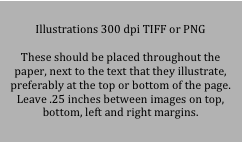
\includegraphics[width=3.31in]{figure.png}
% \caption{This is an example of figure caption. Note that all figures, and tables are to be referenced in the text. \copyright Respect Copyright.}
% \end{figure}

% \begin{figure*}
% 
\includegraphics[width=\textwidth]{two-column-figure.png}
% \caption{Example of a double-column figure with caption. \copyright Respect Copyright.}
% \end{figure*}

\bibliographystyle{isea}
\bibliography{isea}

\section{Bibliography}
The title “Bibliography” should be 12 point, bold style, centred. Using 9 point, regular type, list your bibliography in alphabetical order by family name, after the references. The difference between a reference list and a bibliography is that in your references, you list all the sources you directly referred to in the body of your writing - in numerical order, whereas a bibliography includes an alphabetical listing of all those authors and sources that you have consulted while writing your essay. Use the same format as for the references otherwise.

\section{Author Biography}

The title ``Author(s) Biography(ies)'' should be 12 point, bold style, centered. Using 9 point, regular type, biographies should be no longer than 150-word count.

\end{document}
